\documentclass[a4paper,12pt]{article}
\addtolength{\oddsidemargin}{-1.cm}
\addtolength{\textwidth}{2cm}
\addtolength{\topmargin}{-3cm}
\addtolength{\textheight}{3.5cm}
\makeindex


\usepackage[pdftex]{graphicx}
\usepackage{makeidx}
\usepackage{float}
\usepackage{hyperref}
\hypersetup{
	colorlinks=true,
	linkcolor=blue,
	filecolor=magenta,      
	urlcolor=cyan,
}



% define the title
\author{CodeBlox}
\title{Tender}
\begin{document}
	\setlength{\parskip}{6pt}
	
	% generates the title
	\begin{titlepage}
		\begin{center}
			
\includegraphics[width=1\textwidth]{./Pictures/up_logo.png}\\[1.5cm] 
			\textsc{\LARGE Department of Computer Science} \\ [.5cm]
			\textsc{\Large Functional and Architectural Requirements} \\ [.5cm]
			\line(1,0){450}\\[.5cm]
			\huge{\bfseries Client: Gavin Potgieter}\\
			\line(1,0){450}\\[.5cm]
			\textsc{\LARGE Team: CodeBlox}\\ [0.5cm]
			
			
			\textsc{\large Tshepo Malesela (Bsc: Computer Science)}\\
			\textsc{\large Lorenzo Spazzoli (Bsc: Computer Science)}\\
			\textsc{\large Bilal Muhammad (BIS: Multimedia)}\\
			\textsc{\large Dirk de Klerk (BIS: Multimedia)}\\ [3.9cm]
			
			\large\today
		\end{center}
	\end{titlepage}
	
	\tableofcontents
	\thispagestyle{empty}
	\footnotesize
	\normalsize
	
	
	
	
	\newpage
	\section{Introduction}
	The purpose of this document is to provide a detailed overview of the functional and architectural requirements with regard to the DropOff Project that was assigned to team CodeBlox. The document will be under constant revision, and will change as the project progresses. 
	
	{\noindent}It will provide the development team with a reference that can be used to develope from, thus ensuring that all functional and architectural requirements are met.
	
	{\noindent}The document will also serve as means of communication between the client and development team. Thus any additional requirements from the clients' side can be appended to the document, and has to be adhered to from the development side.
	
	\section{Project Objectives} The \textbf{primary objective} of the project is to create an automated service system that will provide customers with the ability to grant delivery personnel access to a drop safe and/or demarcated area of their home. This will ensure that deliveries to be made can be completed without the need of someone being physically present on the premises.
	
	{\noindent}Initially this will consist of the generation of a One Time Pin (OTP), that will be sent to the delivery personnel, granting them single access to the demarcated area. Once the delivery has been made. The user needs to be able to ensure that the residence is secure.
	
	{\noindent}If time allows it. The system will be expanded to use audio and video communication to validate the identity of the delivery person.
	
	{\noindent}In addition to the functionality of the system, it needs to be as \textbf{cost effective} as possible. This will allow a larger audience to gain access to the system. 
	
	{\noindent}The \textbf{secondary objective} (if time permits) is to make the system scalable. This will enable services to expand to other areas of the home. Thus allowing users an affordable solution to home automation.
	
	\newpage
	\section{Functional Requirements}
	
	\subsection{PersonService}
	The PersonService module will be responsible for maintaining user information. The module will also have the responsibility of storing demographic information about the users, store information about the users' next of kin, and finally keep track of the users account status.
	
	\subsubsection{Scope}
	The scope of the Users module is shown below
	
	
	{\noindent}The scope of the Users module includes
	\begin{itemize}
		\item adding, removing, and modifying users on the system
		\item changing user information
	\end{itemize}
	
	\subsubsection{Domain Model}
	The domain model for the Users module is shown below
	
	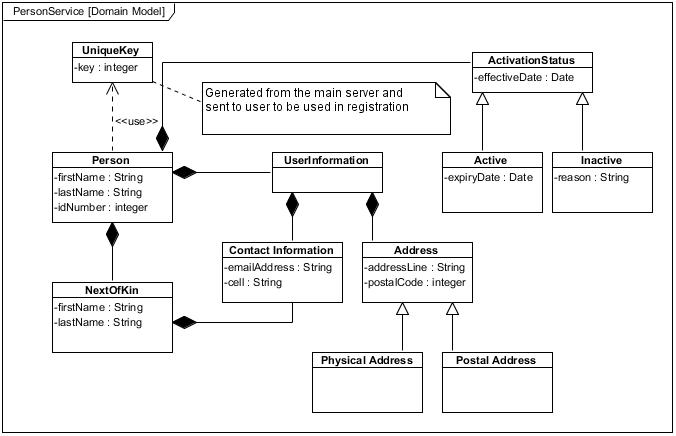
\includegraphics[width=1\textwidth]{./Pictures/UML/PersonServiceDomain.jpg}\\[1.5cm]	

	{\noindent}Each user has a firstname and a lastname, as well as an id number. Each person will also have associated with them UserInformation, which will include email, cellphone, as well as Address. A next of kin will also be available in case the user cannot be reached. Lastly the Person will have associated with it an ActivationStatus, that will determine if the user is still able to receive services.	
	 
	\newpage
	\subsubsection{Use Cases}
	
	\begin{itemize}
		\item \textbf{loginUser} - Allows a user to log into the system.\\[0.5cm]
		\textit{preconditions:}
			\begin{itemize}
				\item The user has already been registered with the system.
				\item The user is still considered an active user.
				\item The user has provided the correct login credentials.
			\end{itemize}
			
		\textit{postconditions:}
			\begin{itemize}
				\item The user is logged into the system.
				\item User gains access to all the services available to him/her.\\[0.5cm]
			\end{itemize}
			
		\item \textbf{logoutUser} - Allows a user to logout of the system.\\[0.5cm]
		\textit{preconditions:}
			\begin{itemize}
				\item The user is already logged into the system.
			\end{itemize}
		
		\textit{postconditions:}
			\begin{itemize}
				\item The user is logged out of the system.
				\item The user no longer has access to the services provided by the system.\\[0.5cm]
			\end{itemize}
			
		\item \textbf{registerUser} - Allows a user to be registered on the system and provide them access to the various services.\\[0.5cm]
		\textit{preconditions:}
			\begin{itemize}
				\item The user does not already exist on the system.
				\item The user has been provided with a unique registration key
			\end{itemize}
		
		\textit{postconditions:}
			\begin{itemize}
				\item The user has been added to the system and may continue.\\[0.5cm]
			\end{itemize}
			
		\item \textbf{updateDetails} - Allows a user to update their information.\\[0.5cm]
		\textit{preconditions:}
			\begin{itemize}
				\item The user exists on the system
				\item The user has to correct credentials
			\end{itemize}
		
		\textit{postconditions:}
			\begin{itemize}
				\item The users' information is updated.
			\end{itemize}
	\end{itemize}
	
	\newpage
	
	\subsection{CameraService}
	The CameraService is responsible for providing the user with access to the live camera feed. The user needs to be able to access a feed, and also needs to be able to close a camera feed. This will ultimately allow them to verify the identity of the delivery person. 
	
	\subsubsection{Scope}
	The scope of the CameraService module is shown below
	
	
	{\noindent}The scope of the CameraService module includes
	\begin{itemize}
		\item Gaining access to the live camera feed.
		\item Close the camera feed as a means to save on bandwidth.
	\end{itemize}
	
	\subsubsection{Domain Model}
	The domain model for the CameraService module is shown below
	
	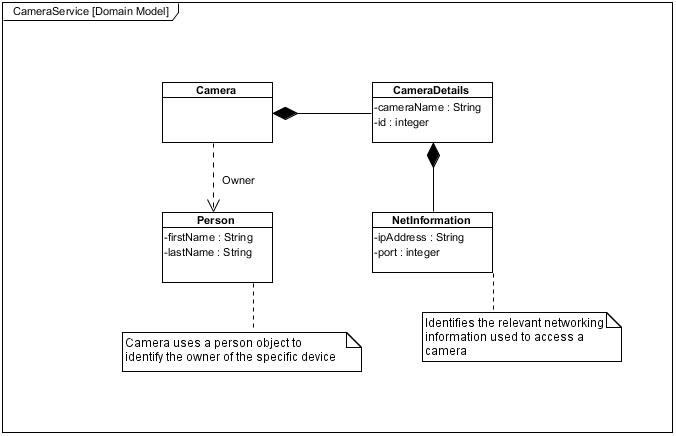
\includegraphics[width=1\textwidth]{./Pictures/UML/CameraServiceDomain.jpg}\\[1.5cm]	
	
	{\noindent}Each Camera will have associated with it CameraDetails that will provide information to how the camera may be accessed. Also the Camera Class will be associated with a Person class to identify them as the owner of the device.
	
	\newpage
	\subsubsection{Use Cases}
	
	\begin{itemize}
		\item \textbf{getCameraFeed} - Enables the user to gain access to the live camera feed.\\[0.5cm]
		\textit{preconditions:}
		\begin{itemize}
			\item The user is still active in the system.
			\item The camera is available to be accessed.
		\end{itemize}
		
		\textit{postconditions:}
		\begin{itemize}
			\item The user receives a live stream.\\[0.5cm]
		\end{itemize}
		
		\item \textbf{closeCameraFeed} - Allows a user to close a camera feed.\\[0.5cm]
		\textit{preconditions:}
		\begin{itemize}
			\item The camera feed is currently streaming.
		\end{itemize}
		
		\textit{postconditions:}
		\begin{itemize}
			\item The camera stops streaming a live feed.\\[0.5cm]
		\end{itemize}
	\end{itemize}
	
	\newpage
	\subsection{PinService}
	The PinService Module is responsible for generating new pins as a backup, should the camera system fail. The module will also need to keep track of the status of the pin i.e. whether or not it has been used or not, as well as its life time. If a pin has been used or it has reached its life time maximum, a new pin has to be generated.
	
	\subsubsection{Scope}
	The scope of the PinService module is shown below
	
	
	{\noindent}The scope of the PinService module includes
	\begin{itemize}
		\item Generating a new pin.
		\item Keeping track of a pins' validity through life time and status.
	\end{itemize}
	
	\subsubsection{Domain Model}
	The domain model for the PinService module is shown below
	
	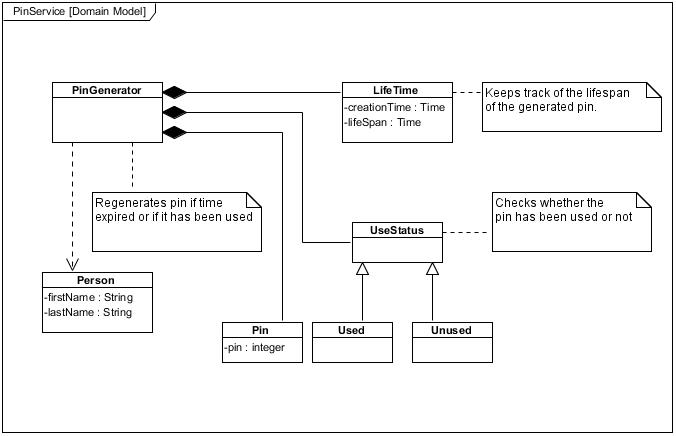
\includegraphics[width=1\textwidth]{./Pictures/UML/PinServiceDomain.jpg}\\[0cm]	
	
	{\noindent}The main class will be the PinGenerator. Associated with each pin generator will be a Pin, which will store the relevant pin that may be used as a fail safe. Also associated with the PinGenerator are the LifeTime and UseStatus classes, which are responsible for monitoring the Pins' validity. The PinGenerator is also associated with a Person so that each generated pin is sent to the correct person.
	
	\newpage
	\subsubsection{Use Cases}
	
	\begin{itemize}
		\item \textbf{generatePin} - The System will generate a new pin to be used as a fail safe.\\[0.5cm]
		\textit{preconditions:}
		\begin{itemize}
			\item A pin has expired.
			\item A pin has already been used.
		\end{itemize}
		
		\textit{postconditions:}
		\begin{itemize}
			\item A new pin is generated.\\[0.5cm]
		\end{itemize}
		
		\item \textbf{displayKeypad} -  The keypad to enter the pin will be displayed.\\[0.5cm]
		\textit{preconditions:}
		\begin{itemize}
			\item The system is making use of the failsafe.
		\end{itemize}
		
		\textit{postconditions:}
		\begin{itemize}
			\item The keypad is displayed on screen.\\[0.5cm]
		\end{itemize}
		
		\item \textbf{updateServer} -  The pin is updated server side for later use.\\[0.5cm]
		\textit{preconditions:}
		\begin{itemize}
			\item A new pin has been generated.
		\end{itemize}
		
		\textit{postconditions:}
		\begin{itemize}
			\item The new pin is reflected on the server.\\[0.5cm]
		\end{itemize}
		
		\item \textbf{getPin} - Allows the user to receive the generated pin.\\[0.5cm]
		\textit{preconditions:}
		\begin{itemize}
			\item The user is logged into the system.
			\item The pin is available.
		\end{itemize}
		
		\textit{postconditions:}
		\begin{itemize}
			\item The pin is sent to the user.\\[0.5cm]
		\end{itemize}
	\end{itemize}
	\newpage
	
	\subsection{LockService}
	The LockService Module will have the responsibility of controlling access to the dropbox. The lock mechanism can be comprised of any suitable technology for example a step motor or magnetic lock. The service should be able to unlock and lock the device, as well as keep track of the device status.
	
	\subsubsection{Scope}
	The scope of the LockService module is shown below
	
	
	{\noindent}The scope of the LockService module includes
	\begin{itemize}
		\item Open up the dropOff box (via unlock or rotate of motor)
		\item Lock the dropOff box
		\item keep track of the devices' status.
	\end{itemize}
	
	\subsubsection{Domain Model}
	The domain model for the LockService module is shown below
	
	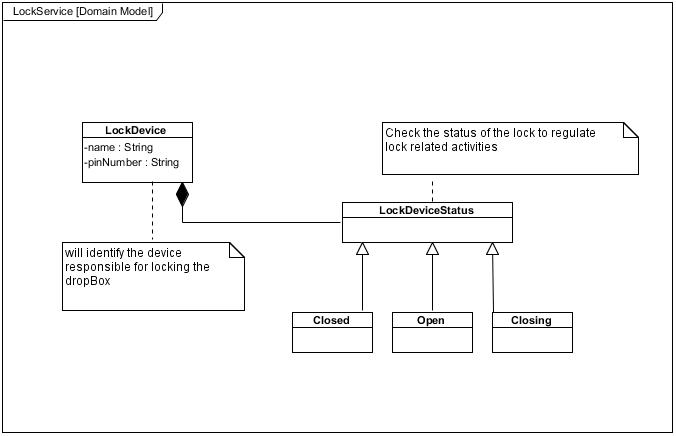
\includegraphics[width=1\textwidth]{./Pictures/UML/LockServiceDomain.jpg}\\[0cm]	
	
	{\noindent}The LockDevice Class consists of a name and a pinNumber. The name is used to identify the device and pinNumber will be used to identify the pin used to interface with the raspberry pi. Associated with the LockDevice class will be a LockDeviceStatus, that will be used to keep track of the devices' current status i.e. Closed, Open, and Closing.
	
	\newpage
	\subsubsection{Use Cases}
	
	\begin{itemize}
		\item \textbf{openDropOff} - Will allow the user to open up the box once identity has been verified.\\[0.5cm]
		\textit{preconditions:}
		\begin{itemize}
			\item The box is closed.
			\item The user is logged in.
			\item The camera feed is accessible (System is functioning normally).
		\end{itemize}
		
		\textit{postconditions:}
		\begin{itemize}
			\item The box is opened up.\\[0.5cm]
		\end{itemize}
		
		\item \textbf{lockDropOff} -  This function will allow the dropOff box to be locked and secured again.\\[0.5cm]
		\textit{preconditions:}
		\begin{itemize}
			\item The device is currently open/unlocked.
		\end{itemize}
		
		\textit{postconditions:}
		\begin{itemize}
			\item The device is locked.\\[0.5cm]
		\end{itemize}
		
		\item \textbf{getDropOffStatus} -  Provides the user/system with state information about the system.\\[0.5cm]
		\textit{preconditions:}
		\begin{itemize}
			\item The system is in some state, either Open, Closed, Closing.
		\end{itemize}
		
		\textit{postconditions:}
		\begin{itemize}
			\item The appropriate state is returned to the system/user.\\[0.5cm]
		\end{itemize}
	\end{itemize}
	\newpage
	
	\subsection{NotificationService}
	The NotificationService Module is responsible for informing the user that a delivery person is at his/her residence. If the home device is unable to communicate with the server, a message has to be displayed locally informing the delivery person to contact the owner to obtain a pin. 
	
	\subsubsection{Scope}
	The scope of the NotificationService module is shown below
	
	
	{\noindent}The scope of the NotificationService module includes
	\begin{itemize}
		\item Send a notification to the user to inform him/her of a potential delivery.
		\item Send a message to the local device to instruct delivery person.
		\item Set and get notification status.
	\end{itemize}
	
	\subsubsection{Domain Model}
	The domain model for the NotificationService module is shown below
	
	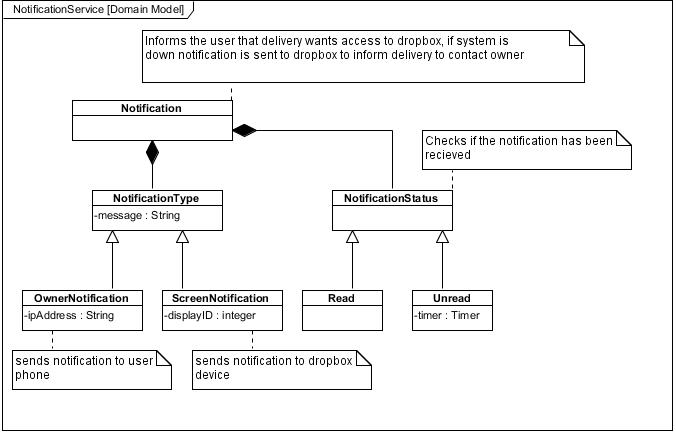
\includegraphics[width=1\textwidth]{./Pictures/UML/NotificationServiceDomain.jpg}\\[0cm]	
	
	{\noindent}
	
	\newpage
	\subsubsection{Use Cases}
	
	\begin{itemize}
		\item \textbf{sendUserNotification} - Will send a notification to the user, informing him/her of a delivery.\\[0.5cm]
		\textit{preconditions:}
		\begin{itemize}
			\item The alert button has been pressed.
			\item The home device is able to communicate with the server.
		\end{itemize}
		
		\textit{postconditions:}
		\begin{itemize}
			\item A notification is sent to the user.\\[0.5cm]
		\end{itemize}
		
		\item \textbf{sendLocalNotification} -  Will generate a message that will be displayed on the local device.\\[0.5cm]
		\textit{preconditions:}
		\begin{itemize}
			\item The alert button has been pressed.
			\item The local device cannot communicate with the server.
		\end{itemize}
		
		\textit{postconditions:}
		\begin{itemize}
			\item A message is displayed on the local device interface.\\[0.5cm]
		\end{itemize}
		
		\item \textbf{setNotificationStatus} -  Allows the status of the sent notification to be set as Read, or Unread.\\[0.5cm]
		\textit{preconditions:}
		\begin{itemize}
			\item A notification has been sent.
		\end{itemize}
		
		\textit{postconditions:}
		\begin{itemize}
			\item The status of the notification is set to Unread. Once read it is set to red.\\[0.5cm]
		\end{itemize}
		
		\item \textbf{getNotificationStatus} -  Provides the user/system with the current status of the notification.\\[0.5cm]
		\textit{preconditions:}
		\begin{itemize}
			\item A notification status has been set.
		\end{itemize}
		
		\textit{postconditions:}
		\begin{itemize}
			\item Returns the status of the notification.\\[0.5cm]
		\end{itemize}
	\end{itemize}
	\newpage
	
	\section{Architectural Requirements/Design Specification}
	
	\subsection{Software architecture overview}
	
	The diagram below provides a high-level overview of the software architecture as a whole. For this particular project we are making use of a layered software architecture, therefore the diagram shows how the respective components of the system will be layered.\\
	
	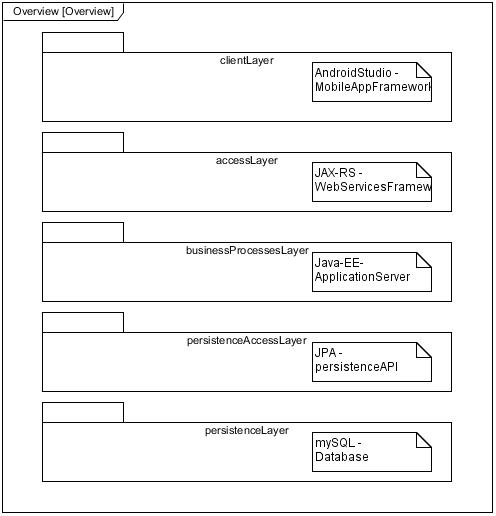
\includegraphics[width=1\textwidth]{./Pictures/UML/architectureOverview.jpg}\\[1.5cm]
	
	
	\subsubsection{clientLayer}
	The layer with which the client will be interacting. This will represent the interface with which the client will be interacting, be it an android or web interface.
	\subsubsection{accessLayer}
	The layer represents the Restful web services layer. It will be used to wrap business process as RESTful services so that multiple access channels may make use of these services. 
	\subsubsection{businessProcessesLayer}
	This layer will host all the business logic within the application server. All methods will be executed server side, and all processes will be hosted on the JBoss server.
	\subsubsection{persistenceAccessLayer}
	This layer represents the Java Persistence API that is used to interact with the database. The client will never interact with the database directly but instead will make use of Entity managers.
	\subsubsection{persistenceLayer}
	This layer refers to the actual database technology that is used for persistence. In this case we will be using a mySQL relational database for persistence.
	
	\subsection{Access Channel Requirements}
	\begin{itemize}
		\item An android application that allows the owner of the property to be notified when someone is outside the premises and to have a full video stream while the person is in the resident.
		
		\item The android application also allows the owner to remotely open and close the premises.
		
		\item The application will also let the owner generate a one-time pin to enable the person to enter the premises (This is the initial system and will be later used as the backup system).  
		
		\item A JFrame touch screen intercom system that allows the delivery person who wants to enter the premises, to enter the pin that was generated by the owner and gain access to the resident.
		
		\item A web application to enable the owner of the property to view recorded camera footage and to configure the camera angles along with system settings. 
	\end{itemize}
	
	\newpage
	\subsection{Architectural Scope}
	\begin{itemize}
		\item Video stream access of the premises from anywhere at any time i.e. constant camera footage of the premises. This will be done using SIP (Session Initiation Protocol).
		
		\item Voice will also be transmitted using SIP, when the delivery person interacts with the intercom system.
		
		\item An internal server that hosts all the devices in the household, allowing for additional devices to be connected at any time. 
		
		\item An external could server to allow communication with the internal server and the android application the owner will be using. 
	\end{itemize}
	
	\subsection{Global Quality Requirements}
	
	\subsubsection{Performance}
	\begin{itemize}
		\item The system has to be stable and responsive enough to send a package with the auto generated pin. The system should also to stable enough to stream video to the android application used by the owner. 
	\end{itemize}
	
	\subsubsection{Security}
	\begin{itemize}
		\item In terms of sending the OTP, end to end encryption with (check best hashing algorithm) will be used. For the initial system (which will be later used as the backup system) the OTP will be sent in a HTTP package. 
		\item The OTP generated will be deleted once used, this ensures that a pin that was used will not work again if the delivery person attempts to use it at a later stage.
		\item In future the system will enforce confidentiality through encrypted communication of SIP (Session Initiation Protocol).
		\item Users of the system will will also need to be authenticated before they may make use of the various processes.
		\item Certain functionality will be restricted to the authorisation of a user, i.e. what role the user has within the system.
	\end{itemize}
	
	\subsubsection{Reliability}
	\begin{itemize}
		\item The property owner should be able to access the residence at any time using the android application 
		\item The user should be able to grant access at any time using the application
		\item With regards to the backup system, the user should be able to generate a pin from anywhere and the pin should work by granting access to the delivery person. 
		\item The response of the gate opening when the user opens it using the application should be reasonable.
	\end{itemize}
	
	\subsubsection{Flexibility}
	\begin{itemize}
		\item The user should be able to access the application from any of his/her devices.
		\item The application should be able to run smoothly on any android device that is Android 4.0 and above.
	\end{itemize}
	
	\subsubsection{Maintainability}
	\begin{itemize}
		\item Maintenance of this application will be handled by the developers, hence the use of an external server.
		\item The server will have to be well maintained because all the people who have this system in their homes will connect to the external server. 
		\item Developers should be able to to add new functionality to the system, as well as change some if the existing functionality if they wish.
	\end{itemize}
	
	\subsubsection{Monitorability}
	\begin{itemize}
		\item While the delivery person is on the premises the owner of the property keeps track of all the activities on the resident. 
		\item When there is no one on the resident, the cameras monitor all movement on the premises.  
	\end{itemize}
	
	\subsubsection{Usability}
	\begin{itemize}
		\item The application should be simple enough for the user to use it without any training. 
		\item The application should have basic instructions to ensure that the user is 100\% sure of the action they are performing.
	\end{itemize}
	
	\subsubsection{Cost}
	\begin{itemize}
		\item The cost of the system should be kept to a minimum and made as affordable as possible. 
		\item This system will mainly use Raspberry pis, keeping the development costs low. 
	\end{itemize}
	
	
	\subsubsection{Testability}
	\begin{itemize}
		\item The individual components of the system needs to be testable through the use of mock objects and automated unit tests.
		\item Automated integration tests should be used to test the system as a whole.
		\item In particular the tests need to verify that the preconditions are met, and that post conditions hold true once a service has been provided.
	\end{itemize}
	
	\subsection{Architectural Constraints}
	The client has some architectural specifications in place that will need to be adhered to, in order to successfully complete this project.
	
	\subsubsection{Use of Inexpensive Devices}
	The devices used to construct the physical system needs to be as inexpensive as possible, thus providing a larger audience with access to it. Devices such as the following will be included:
	\begin{itemize}
		\item Raspberry Pi 3
		\item IP Camera/Pi Camera
		\item Internet Enabled Switches
		\item WiFi Routers
		\item Android Smartphone (Users are assumed to posses one already).
	\end{itemize}
	
	\subsubsection{Technology Stack}
	For monetary reasons, the client has requested that the entire system be developed using open source technologies. CodeBlox has therefore decided to settle on the Java Ecosystem, since we have already had exposure to such technologies. a Preliminary stack will include the following technologies:
	
	\begin{itemize}
		\item \textbf{Java EE} as the primary development platform
		\item \textbf{NetBeans IDE} as the primary development environment.
		\item \textbf{Android Studio} to the build the mobile application that will be used.
		\item \textbf{Apache Maven} will be used as the primary build tool
		\item \textbf{Mockito/TestNG} for unit testing
		\item \textbf{JAX-RS} for implementing RESTful webservices.
		\item \textbf{JBoss} for the primary application server (New version of glassfish seems to have some issues).
		\item \textbf{Linux} as the operating system
		\item \textbf{MySQL} as the primary persistence technology.
	\end{itemize}
	
	\subsection{Architectural Design}
	This section specifies the architectural responsibilities of various architectural components.
	\subsubsection{Architectural Responsibilities}
	\begin{itemize}
		\item The responsibility of providing an execution environment for business processes is assigned to an application server. i.e. \textbf{JBoss}
		\item The responsibility of persisting domain objects is assigned to the the database i.e. \textbf{MySQL}
		\item The responsibility of providing access to the database is assigned to the persistence API i.e. \textbf{Java Persistence API (JPA)}
		\item The responsibility of providing access channels to users is assigned to the web services framework i.e. \textbf{Jersey, which is an implementation of JAX-RS for RESTful Web Services}
		\item The responsibility of providing users access via mobile devices is assigned to the mobile application framework i.e. \textbf{Android Studio}
	\end{itemize}
	
	\subsubsection{Infrastructure}
	For this particular project, the \textbf{layered architectural pattern} will be used as an infrastructure. The pattern limits access of components within one layer to components which are in the same layer or one level down. Thus it cannot access components in the layer above it. What makes it a very useful pattern is that different levels can be easily replaced without disrupting layers either above or below it. 
	
	\newpage
	\subsection{Application Server}
	The application server refers to the architectural component within which business processes are deployed and executed. Put in other words, the application server will be hosting the business processes layer of the system.
	
	\subsubsection{Quality Requirements}
	\begin{itemize}
		\item\textbf{Flexibility}
		\begin{itemize}
			\item deploy different versions of the system with minimum downtime.
		\end{itemize}
		
		\item\textbf{Reliability}
		\begin{itemize}
			\item Requires that service requests are not partially executed. Thus the requested service will only be executed once postconditions are fulfilled. If a service could not be provided, a reason must be given.
		\end{itemize}
		
		\item\textbf{Security}
		\begin{itemize}
			\item The application server must support role-based authorisation. Thus only a user with a certain level of authorisation may execute certain processes. No direct access should be provided to the database. 
		\end{itemize}
		
		\item\textbf{Testability}
		\begin{itemize}
			\item The application server should support out-of-container testing as well as unit testing.
		\end{itemize}
		
	\end{itemize}
	
	\subsubsection{Tactics as provided by Java EE}
	Java EE 7 supports all of the architectural tactics which are specified in the software architecture specific to the application server.
	
	\begin{itemize}
		\item\textbf{Flexibility Tactics}
		\begin{itemize}
			\item Context and Dependency Injection (CDI) is fully supported by Java-EE by using the @Injection annotations.
			\item Hot deployment is supported by the \textbf{JBoss} application server.
		\end{itemize}
		
		\item\textbf{Reliability Tactics}
		\begin{itemize}
			\item Java-EE supports container-managed transactions across multiple transaction-supporting resources. Transaction requirements can be specified by annotating services with TransactionAttribute.Required.
		\end{itemize}
		
		\item\textbf{Security}
		\begin{itemize}
			\item Java-EE supports role-based authorisation in the form of container managed declarative authorisation and programmatic authorisation. Methods are annotated with the required security roles.
		\end{itemize}
		
		\item\textbf{Testability}
		\begin{itemize}
			\item Java-EE supports dependency injection and Java-EE specific information is specified via annotations. All application code can thus be executed outside containers. Dependency injection can be used to inject mock objects allowing unit tests to be reused.
		\end{itemize}
		
	\end{itemize}
	\subsection{Database}
	For this particular project we will be utilising a relational database, namely \textbf{MySQL}. Support for the MySQL database is well documented and most developers are fairly familiar with it and its use. 
	
	\subsection{Persistence API}
	The persistence API will provide indirect access to the MySQL database. For the particular project the Java Persistence API will be used.
	
	{\noindent}JPA implements the following:
	\begin{itemize}
		\item\textbf{object-relational mapping}
		\item\textbf{query mapping}
		\item\textbf{object caching}
		\item\textbf{transaction support}
		\item\textbf{connection pooling}
	\end{itemize}
	
	{\noindent}For all query purposes, the Java Persistence Query Language (JPQL) will be used.
	
	\subsection{Web Services Framework}
	The web services framework refers to a wrapping layer that are used to wrap all business processes. This allows for the decoupling of user-interface technologies (in this case android app or web page) from the back end technologies.
	
	\subsubsection{Architecture Design}
	The project will make use of the Jersey implementation of JAX-RS of the JAVA-EE application server. Marshalling and demarshalling will be achieved by making use of the relevant annotations i.e. @produces and @consumes.
\end{document}
